% The Navier-Stokes equations

% \section{The kinematics of flow}
% \subsection{Vorticity}
% \subsection{The Helmholtz decomposition}
% \subsubsection{The stream function}
% \subsubsection{The velocity potential}

\section{Introduction}
% <<<
The incompressible Navier-Stokes equations model the motion of a common kind of viscous fluid called a \textit{Newtonian fluid}.
They are:
\begin{itemize}
\item The Cauchy momentum equation \eqref{cauchy_continuity_differential_material} for constant mass density $\rho$ and velocity $u$,
\item an incompressibility constraint $\nabla\cdot u = 0$ and unknown pressure $p$,
\item and a concrete constitutive relation for the deviatoric stress $\tau$.
\end{itemize}
In anticipation, their common form is
\begin{equation}\label{navier_stokes}
    \rho\frac{Du}{Dt} = - \nabla p + \nabla\cdot\tau + \rho g,\quad \nabla\cdot u = 0,
\end{equation}
where $\tau$ is defined by Stokes' constitutive relation
\begin{equation}\label{stokes_constitutive_relation}
    \tau = \mu\left(\nabla u + \nabla u^T\right),
\end{equation}
where $\mu$ is called the \textit{viscosity}, and $\nabla u$ is the velocity gradient defined in section \ref{deformation_and_velocity_gradients},
measuring the local deformation of a small control volume under
the flow of $u$. We will assume their domain is a subset of $\mathbb{R}^d$, where typically $d = 2$ or $3$, although the Navier-Stokes equations can be solved
in curved domains (see \cite{stam}).
Alongside a domain and appropriate initial and boundary conditions, the Navier-Stokes equations \eqref{navier_stokes}
form a concrete flow problem which
can be solved numerically, or in special situations analytically.
% >>>

\section{Constitutive relations for the Navier-Stokes equations}
% <<<
We begin with the standard conservation equations of mass and linear momentum, \eqref{conservation_system}:
\begin{equation*}
\begin{split}
    \frac{D\rho}{Dt} + \rho\nabla\cdot u = 0 &\quad\text{(Conservation of mass)},
    \\
    \rho\frac{Du}{Dt} = \rho g + \nabla\cdot\sigma &\quad\text{(Conservation of linear momentum)}.
\end{split}
\end{equation*}
As discussed in section \ref{constitutive_relations}, we need to specify $\sigma$ such that the system is well-formed. Firstly, we replace the
conservation of mass equation with the incompressibility constraint
\begin{equation*}
    \nabla \cdot u = 0.
\end{equation*}
Assuming a constant mass density $\rho$, this also expresses mass conservation. This will preclude phenomena such as acoustic waves in the fluid,
but is a good approximation for many studies of fluid motion (see Batchelor \cite{batchelor}).

\subsection{Conservation of angular momentum}
Angular momentum is traditionally presented in terms of rigid bodies, bodies subject to a distance-preserving constraint between
material points. It is the moment of linear momentum.

The discussion in section \ref{material_points} indicates that we can think of a very small rigid body at a material point, subject to the flow.
This will be subject to a ``spin force''.

Let the material point be $c \in \mathbb{R}^d$, which will act as a ``centre of mass', and let $c \in \Omega_0$.
Define $\bar{x} \coloneqq x - c$.
Define the moment of linear momentum as
\begin{equation}\label{moment_of_linear_momentum}
    \int_{\omn} \bar{x} \wedge \left(\rho u\right)\,dx.
\end{equation}
The symbol $\wedge$ indicates the cross product, whose value should be thought of as a pseudo-vector or ``plane with magnitude''.
We will call this the angular momentum of the control volume $\omn$.
We repeat here an integral form of linear momentum conservation, which already must hold:
\begin{equation}\label{linear_momentum_for_angular}
    \int_{\omn(0)} \Part{(\rho u)}{t}\,dx + \int_{\pomn(0)} \rho u (u\cdot \hat{n})\,dx
    = \int_{\omn(0)} \rho g\,dx + \int_{\pomn(0)} \sigma \hat{n}\,dx.
\end{equation}
It is simple to derive an angular momentum conservation equation, just by taking moments of each vector quantity:
\begin{equation}\label{moment_of_linear_momentum_sources}
    \int_{\omn(0)} \bar{x} \wedge \Part{(\rho u)}{t}\,dx + \int_{\pomn(0)} \bar{x} \wedge \left(\rho u\right)\left(u\cdot \hat{n}\right)\,dx
    = \int_{\omn(0)} \bar{x} \wedge \left(\rho g\right)\,dx + \int_{\pomn(0)} \bar{x} \wedge \left(\sigma \hat{n}\right)\,dx.
\end{equation}
(This precludes the introduction of surface and body couples which induce no linear momentum but do induce angular momentum
\cite{leal}. We ignore these torques.)
\\
If \eqref{linear_momentum_for_angular} holds, should \eqref{moment_of_linear_momentum_sources} hold automatically?

(... figure)
\begin{center}
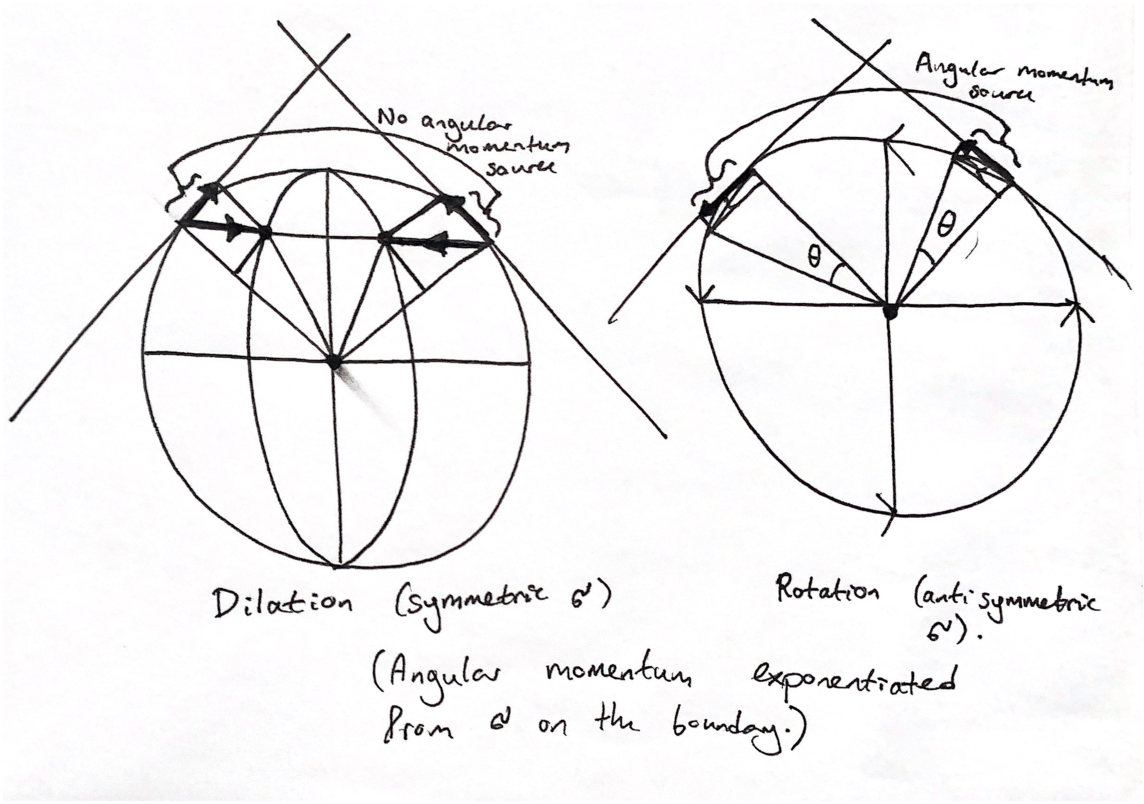
\includegraphics[page=1,width=0.7\linewidth]{figures/3.pdf}
\end{center}


% If the control volume follows the flow, the Reynolds transport theorem \eqref{reynolds_transport_theorem} gives a rate of change of angular momentum:
% \begin{equation}\label{moment_of_linear_momentum_reynolds}
%     \frac{d}{dt}\eval{\left[\int_{\omn(t)} \bar{x} \wedge \left(\rho u\right)\,dx\right]}_{t=0}
%     % = \int_{\omn(0)} \left(x - c\right)\wedge \left(\rho g\right)\,dx + \int_{\pomn(0)} \left(x - c\right) \wedge \hat
%     = \int_{\omn(0)} \bar{x} \wedge \Part{(\rho u)}{t}\,dx + \int_{\pomn(0)} \bar{x} \wedge \rho u (u\cdot \hat{n})\,dx.
% \end{equation}
% The source terms of linear momentum are body forces $\rho g$ on the interior and tractions $\hat{t}$ on the boundary.
% Therefore we have an explicit equation for the rate of change of angular momentum, which we equate to the right-hand-side of
% \eqref{moment_of_linear_momentum_reynolds}:
% \begin{equation}\label{moment_of_linear_momentum_sources}
%     \int_{\omn(0)} \bar{x} \wedge \Part{(\rho u)}{t}\,dx + \int_{\pomn(0)} \bar{x} \wedge \rho u (u\cdot \hat{n})\,dx
%     = \int_{\omn(0)} \bar{x} \wedge \left(\rho g\right)\,dx + \int_{\pomn(0)} \bar{x} \wedge \left(\sigma \hat{n}\right)\,dx.
% \end{equation}
% By the Euler-Cauchy stress principle (section \ref{stress_principle}), we have let the traction $\hat{t} = \sigma \hat{n}$.
% For comparison, we repeat here an integral form of linear momentum conservation, which already must hold:
% \begin{equation*}
%     \int_{\omn(0)} \Part{(\rho u)}{t}\,dx + \int_{\pomn(0)} \rho u (u\cdot \hat{n})\,dx
%     = \int_{\omn(0)} \left(\rho g\right)\,dx + \int_{\pomn(0)} \sigma \hat{n}\,dx.
% \end{equation*}

% >>>

\section{Scaling and dimension}
% <<<
\subsection{The Reynolds number}
% >>>

\section{Stokes flow and the meaning of pressure}\label{pressure_derivation}
% <<<
If we assume that the advective term $u\cdot \nabla u$ in the incompressible Navier-Stokes equations is ``small'',
we can ignore it and derive the linear \textit{unsteady Stokes equations}:
\begin{equation}\label{unsteady_stokes}
    \rho\Part{u}{t} = \mu\Delta u + \rho g - \nabla p, \quad \nabla\cdot u = 0.
\end{equation}
We are assuming validity for low Reynolds number $Re \ll 1$, where convective behaviour is neglible compared to the viscous forces, which for a
Navier-Stokes fluid ``diffuse'' the linear momentum. Setting the left-hand-side of \eqref{unsteady_stokes} to zero results in the \textit{steady Stokes equations}
\begin{equation}\label{steady_stokes}
    \mu\Delta u + \rho g - \nabla p = 0,\quad \nabla\cdot u = 0.
\end{equation}
Time-dependent equation \eqref{unsteady_stokes} can be thought of as a ``gradient descent'' to find the steady Stokes flow \eqref{steady_stokes}.
The steady Stokes equation is a constrained vector Poisson equation, where we have introduced pressure $p$ explicitly.
It is well-known, by Dirichlet's principle, that we can think
of a weak solution to the unconstrained vector Poisson equation as a minimiser of the Dirichlet energy,
\begin{equation}
\begin{aligned}
& \underset{u}{\text{minimize}}
& & E(u) =  \frac{\mu}{2} \inner{\nabla u, \nabla u} - \inner{u, \rho g}.\\
\end{aligned}
\end{equation}
\newcommand{\energygradient}{\frac{\delta E}{\delta u}}
We can validate this by computing the Euler-Lagrange equations:
\begin{align*}
    % \frac{\delta E}{\delta u} = \Part{\fancyL}{u} - \frac{d}{dx}\Part{\fancyL}{\nabla u}
    % notation?
    \frac{\delta E}{\delta u} = \Part{\fancyL}{u} - \frac{d}{dx}\Part{\fancyL}{u_x}
                              = -\rho g - \mu\Delta u = 0.
\end{align*}
We now introduce the incompressibility constraint $\nabla \cdot u = 0$, giving the constrained minimization
\begin{equation}\label{stokes_flow_optimization}
\begin{aligned}
& \underset{u}{\text{minimize}}
& & E(u) =  \frac{\mu}{2} \inner{\nabla u, \nabla u} - \inner{u, \rho g}\\
& \text{subject to}
& & \nabla\cdot u = 0.
\end{aligned}
\end{equation}
It is not immediately obvious how to form the constrained Euler-Lagrange equations here, as $\nabla\cdot$ is a differential operator.
We cannot just write
    $$\text{``}\frac{\delta E}{\delta u} = \lambda\nabla\cdot\text{''}$$
for scalar function $\lambda$, as we can with a pointwise linear constraint such as $u\cdot v = 0$ for some vector field $v$. However, this is just a problem of
notation. The evaluation of energy change with perturbations is defined as
\begin{align*}
    \inner{\frac{\delta E}{\delta u}, \delta u} = \int_\Omega \frac{\delta E}{\delta u}\cdot\delta u\,dx.
\end{align*}
We want this measure of energy change to be purely a divergence measure, up to a scalar multiplier $\lambda$:
\begin{equation}\label{el_pressure_constrained_div}
    \int_\Omega \frac{\delta E}{\delta u}\cdot\delta u\,dx = \int_\om \lambda \nabla\cdot \delta u\,dx.
\end{equation}
This means
that virtual displacements with $\nabla\cdot\delta u = 0$ will not cause an energy change, which is the condition that
we want for a stationary point.
We can now apply integration by parts to \eqref{el_pressure_constrained_div}, assuming that $\delta u$ vanishes on the boundary of the domain, to get
\begin{equation}
    \int_\Omega \frac{\delta E}{\delta u}\cdot\delta u\,dx = -\int_\om \nabla\lambda \cdot \delta u\,dx.
\end{equation}
We can now reasonably apply the localisation step to get the constrained Euler-Lagrange equations
\begin{equation}
\begin{split}
           \frac{\delta E}{\delta u} = -\nabla \lambda
    \quad\equiv\quad \mu\Delta u + \rho g - \nabla \lambda = 0.
\end{split}
\end{equation}
Along with the constraint $\nabla\cdot u = 0$, this is just the steady Stokes equations \eqref{steady_stokes}, where $\lambda = p$! We can see that the pressure $p$
is actually
a Lagrange multiplier, which measures a virtual force that responds to virtual displacements which would break the constraint of incompressibility.
In fact, we may think of this as a derivation of the pressure.

\subsubsection{Alternative direct derivation in terms of a modified energy}
Previously, we emphasized the meaning of the Lagrange multiplier. One utility of Lagrange's methods is their automated calculational power.
It is standard to express that a solution to the optimization
problem \eqref{stokes_flow_optimization}, with a differentiable equality constraint, is a stationary point of the modified energy
\begin{equation}\label{stokes_flow_modified_energy}
    L(u, \lambda) \coloneqq \frac{\mu}{2} \inner{\nabla u, \nabla u} - \inner{u, \rho g} - \inner{\lambda, \nabla\cdot u}.\\
\end{equation}
We can take an evaluated first variation with respect to $u$ to get
\begin{align*}
    \inner{\frac{\delta L}{\delta u}, \delta u} = \inner{-\rho g - \mu\Delta u, \delta u} - \inner{\lambda, \nabla\cdot\delta u},
\end{align*}
which by integration by parts becomes
\begin{equation}
    \inner{\frac{\delta L}{\delta u}, \delta u} = \inner{-\rho g - \mu\Delta u + \nabla \lambda, \delta u}.
\end{equation}
We then get
\begin{equation}
\begin{split}
    \frac{\delta L}{\delta u} &= -\rho g - \mu\Delta u + \nabla \lambda = 0,\\
    \frac{\delta L}{\delta \lambda} &= -\nabla\cdot u = 0,
\end{split}
\end{equation}
which are the steady Stokes equations \eqref{steady_stokes} with pressure $p = \lambda$.



\subsection{Application to hydrostatics}
For example, we may imagine the steady Stokes equations modelling a calm sea with a flat seabed.
We can let the body force be gravity described by a potential $\phi$:
    $$\rho g = -\nabla \phi.$$
If we make a perturbed displacement of the velocity field at the bottom of the ocean, supposing that some volume of water
is beginning to expand,
we are working against gravity as well as our virtual force, pressure.

\vskip 0.2in
(draw this)
\vskip 0.2in

% >>>

% Navier-Stokes in expanded differential form for Cartesian coordinates. Maybe useful for finite differences.
% Working backwards to the weak form doesn't make much sense.
% \subsection{Kinds of fluids}
% \subsubsection{Incompressible fluids}
% \subsubsection{Inviscid flow}
% \subsubsection{Irrotational flow}
% \subsubsection{Steady flow}
% \subsubsection{Viscous flow and Newtonian fluids}

